\documentclass[12pt,a4paper,oneside]{article}
\usepackage[colorlinks=true]{hyperref}
\usepackage[utf8]{inputenc}
\usepackage[english]{babel}
\usepackage{graphicx}
\usepackage{pdfpages}
\textwidth 16cm \textheight 25cm
\topmargin -1.3cm 
\oddsidemargin 0cm
\usepackage{footnote}
\pagestyle{empty}
\begin{document}
\title{Software Defined Receiver SDRX01B not only for radioastronomy}
\author{Jakub Kákona, kaklik@mlab.cz }
\maketitle

\begin{abstract}
This paper describe a design of Software Defined Receiver suitable for radioastronomy purposes. The receiver which has been developed in this project replacing old analog constructions such as RadioJOVE and others.
\end{abstract}

\begin{figure} [htbp]
\begin{center}
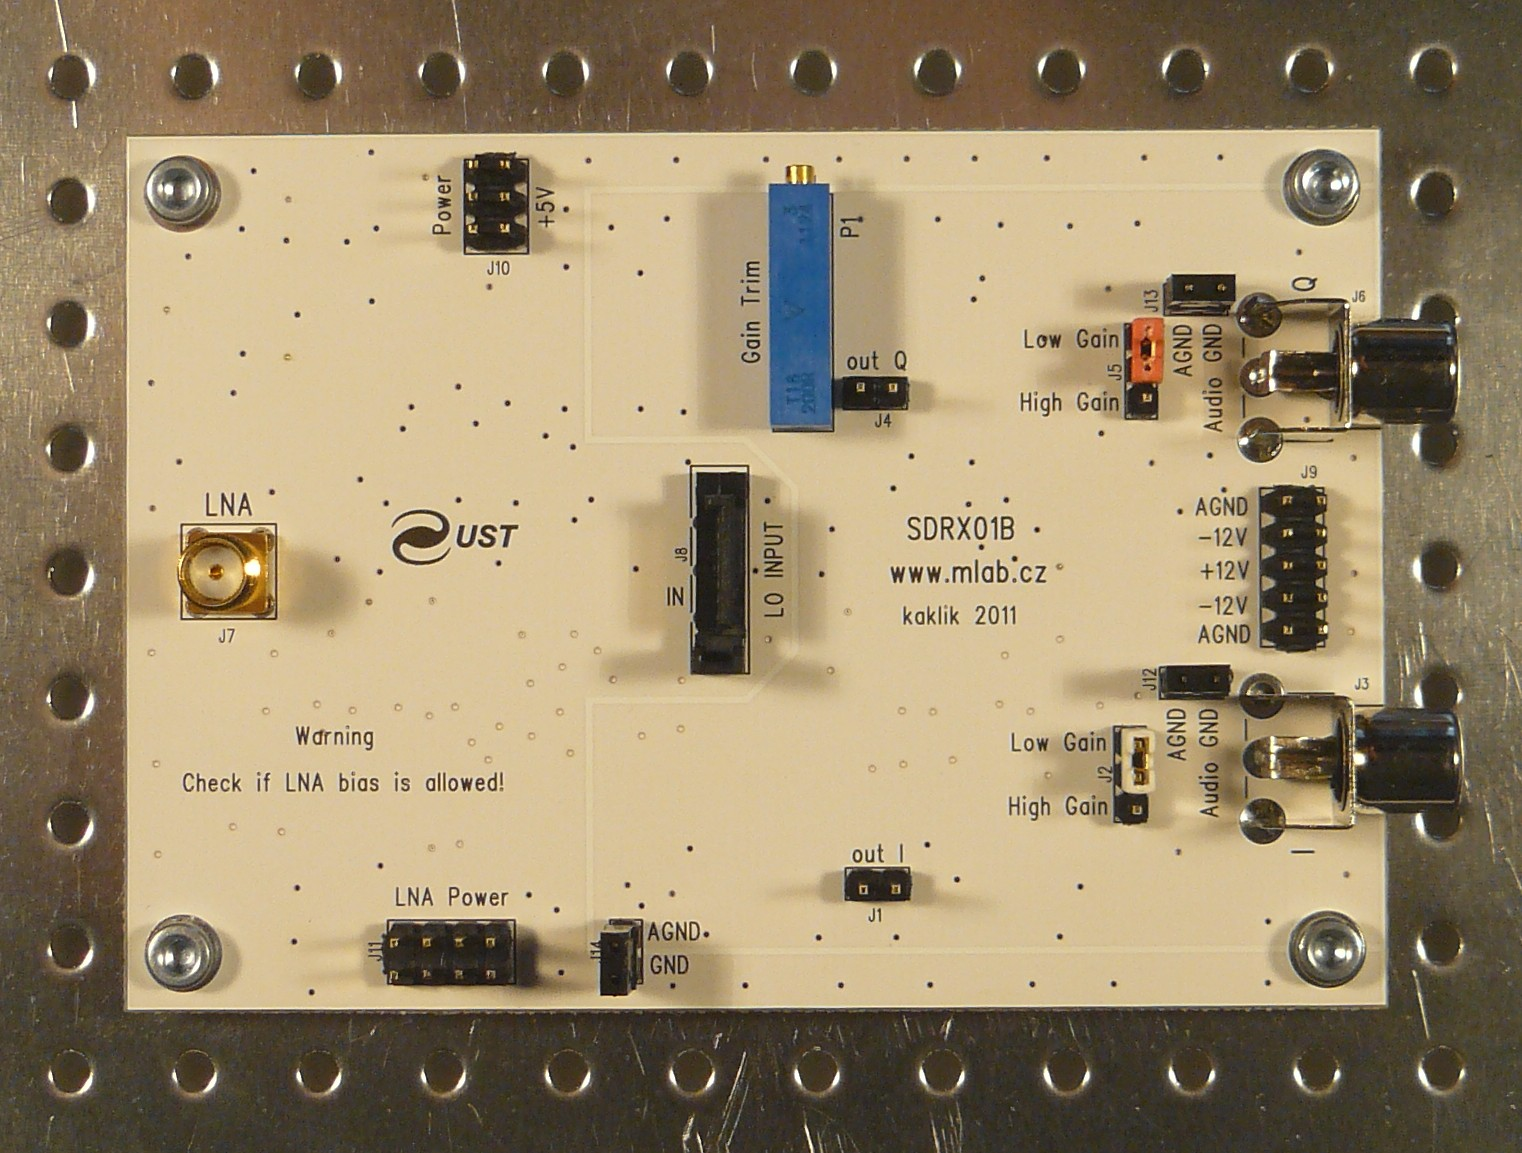
\includegraphics [width=80mm] {./img/SDRX01B_Top_Big.JPG} 
\end{center}
\end{figure}

\begin{figure} [b]

\includegraphics [width=25mm] {./img/SDRX01B_QRcode.png} 
\end{figure}

\newpage
\tableofcontents

\section{Technical parameters}
\begin{savenotes}
\begin{table}[htbp]
\begin{center}
\begin{tabular}{|c|c|p{5cm}|}
\hline
\multicolumn{1}{|c|}{Parameter} & \multicolumn{1}{|c|}{Value} & \multicolumn{1}{|c|}{Note} \\ \hline
Power voltage for analog circuits & $\pm$12 V 100mA \footnote{First devices manufactured before 1.8.2011 may be equipped by 10 V tatal capacitors onl thus cannot by longly stressed by $\pm$12 V power voltage } &  Typical current draw 30 mA \\ \hline
Powering voltage for digital part & +5V &  300mA \\ \hline
Bias of optional LNA & up to +20V max 500mA &   Fused by 750mA on board \\ \hline
Frequency range  & 0,5 - 200 MHz & With populating by chosen parts even up 450MHz \\ \hline
IIP3  & $>$ 0dB & Preliminary \\ \hline
Gain & 40-60dB & Selectable by jumper \\ \hline
Self noise number & $<$ 30dB & \\ \hline
\end{tabular}
\end{center}
\end{table}
\end{savenotes}

\newpage
\section{Description of construction}

\subsection{Circuit}
Construction  of the receiver is delivered from the DR2G receiver \cite{DR2G} which uses CMOS components completely. The main change in this construction is a local oscillator input circuit which allow to receiver work at higher frequencies, because this construction do not divide the input frequency by 4, such as original construction but only by 2. In addition there was be replaced switches in the sampling mixer by faster type and board layout was optimized for higher frequencies and better noise rejection.

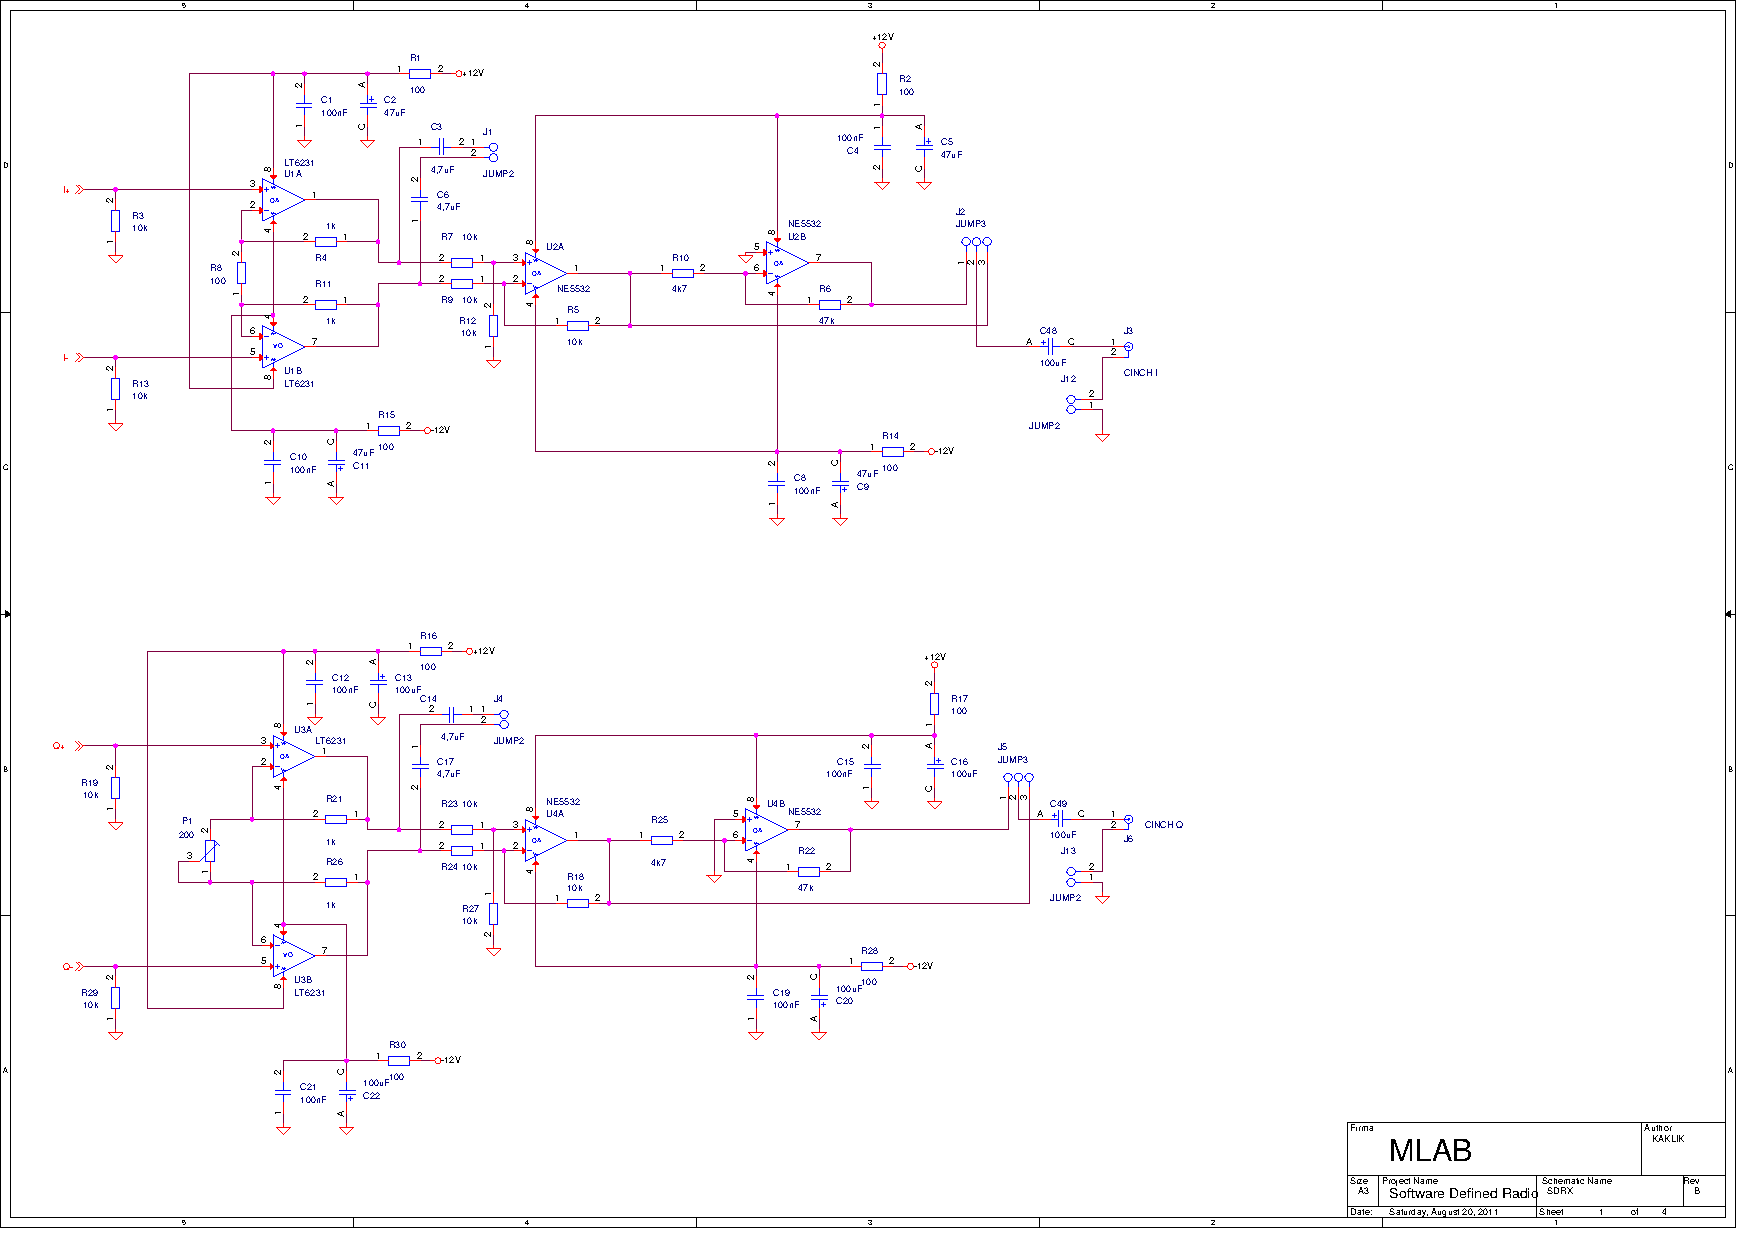
\includepdf[pages={1,2,3,4},landscape=true]{../../SCH/sdrx.pdf}

The necessary part of the receiver is a Local Oscillator (LO), which must be connected to receiver via SATA cable. The LO may be a CLKGEN01B module populated by the 570ABB000107DG chip. SATA cable should be as short as possible to minimize ground loops.

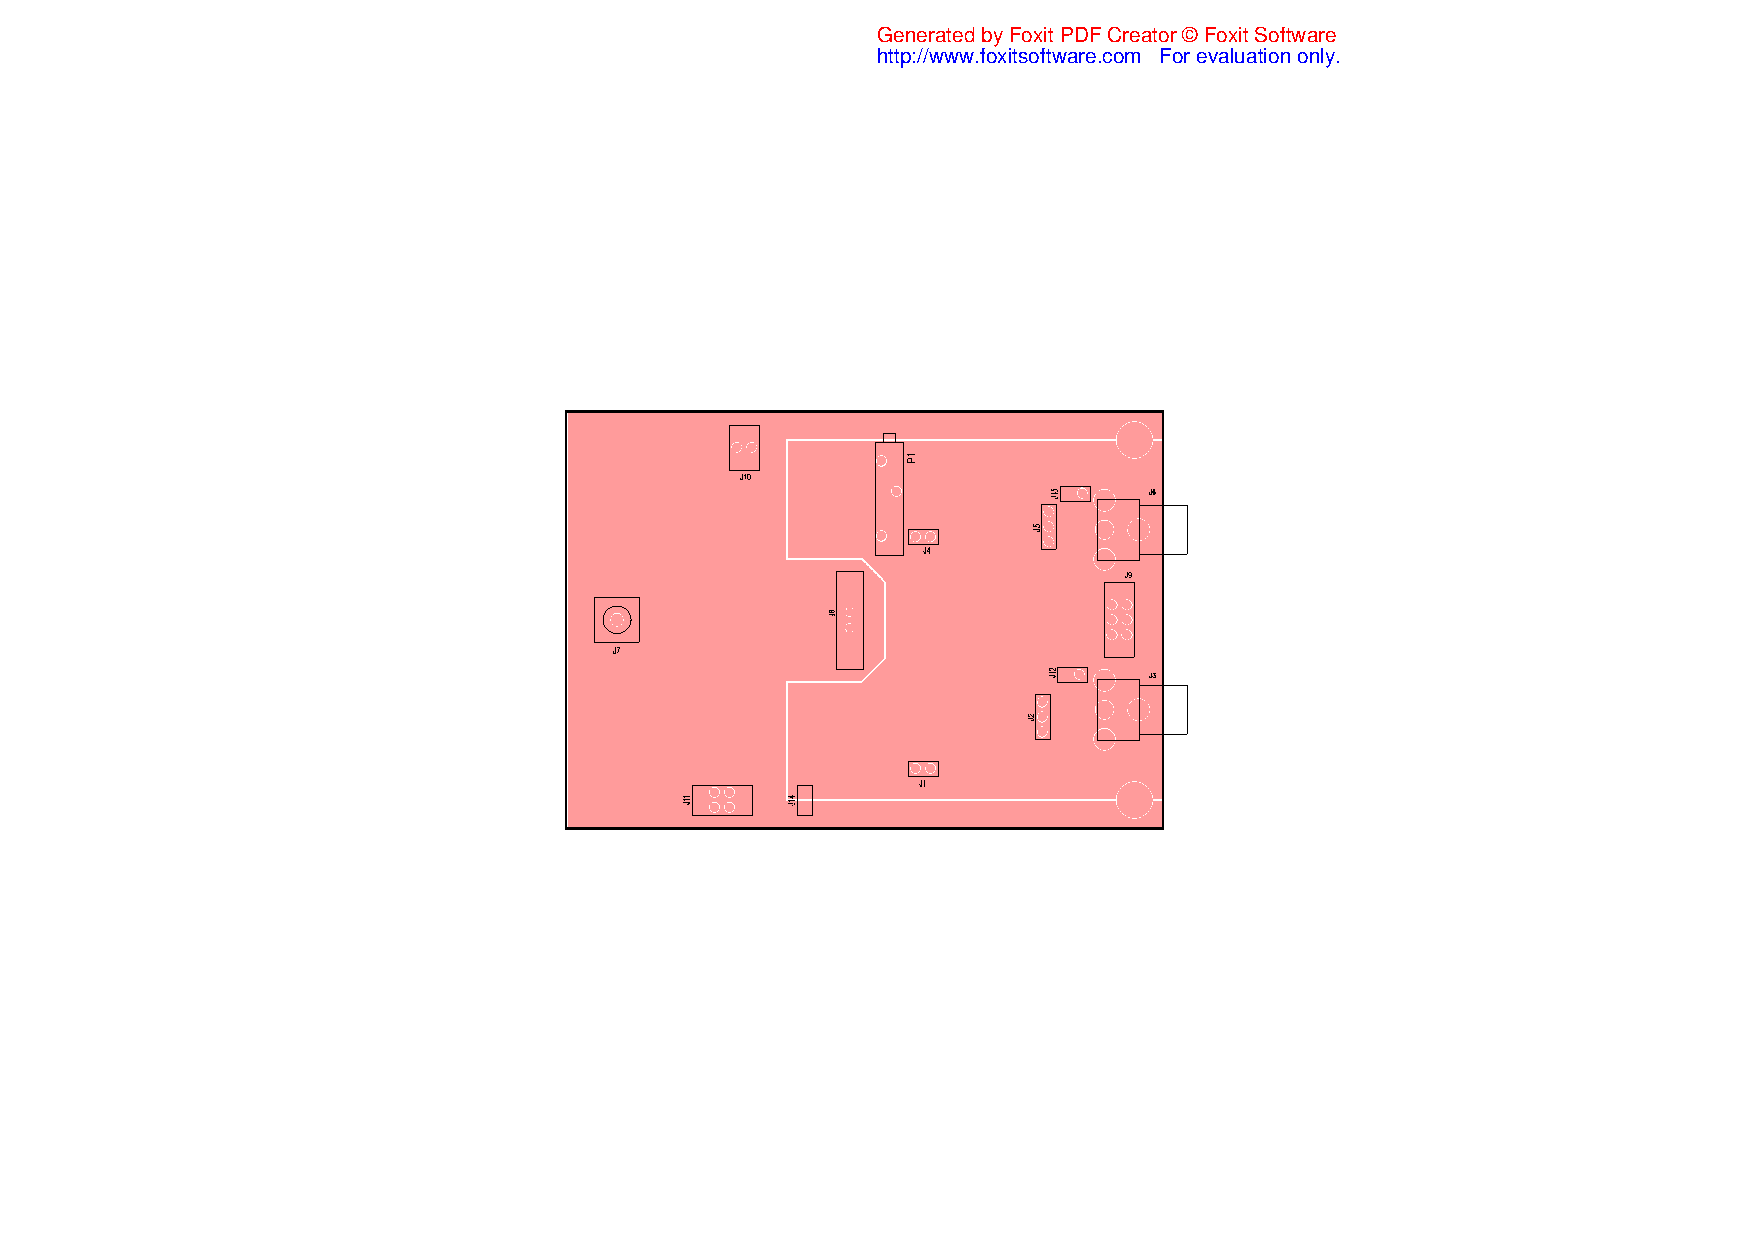
\includepdf[pages={1},landscape=true]{../../CAM_DOC/O1.pdf}

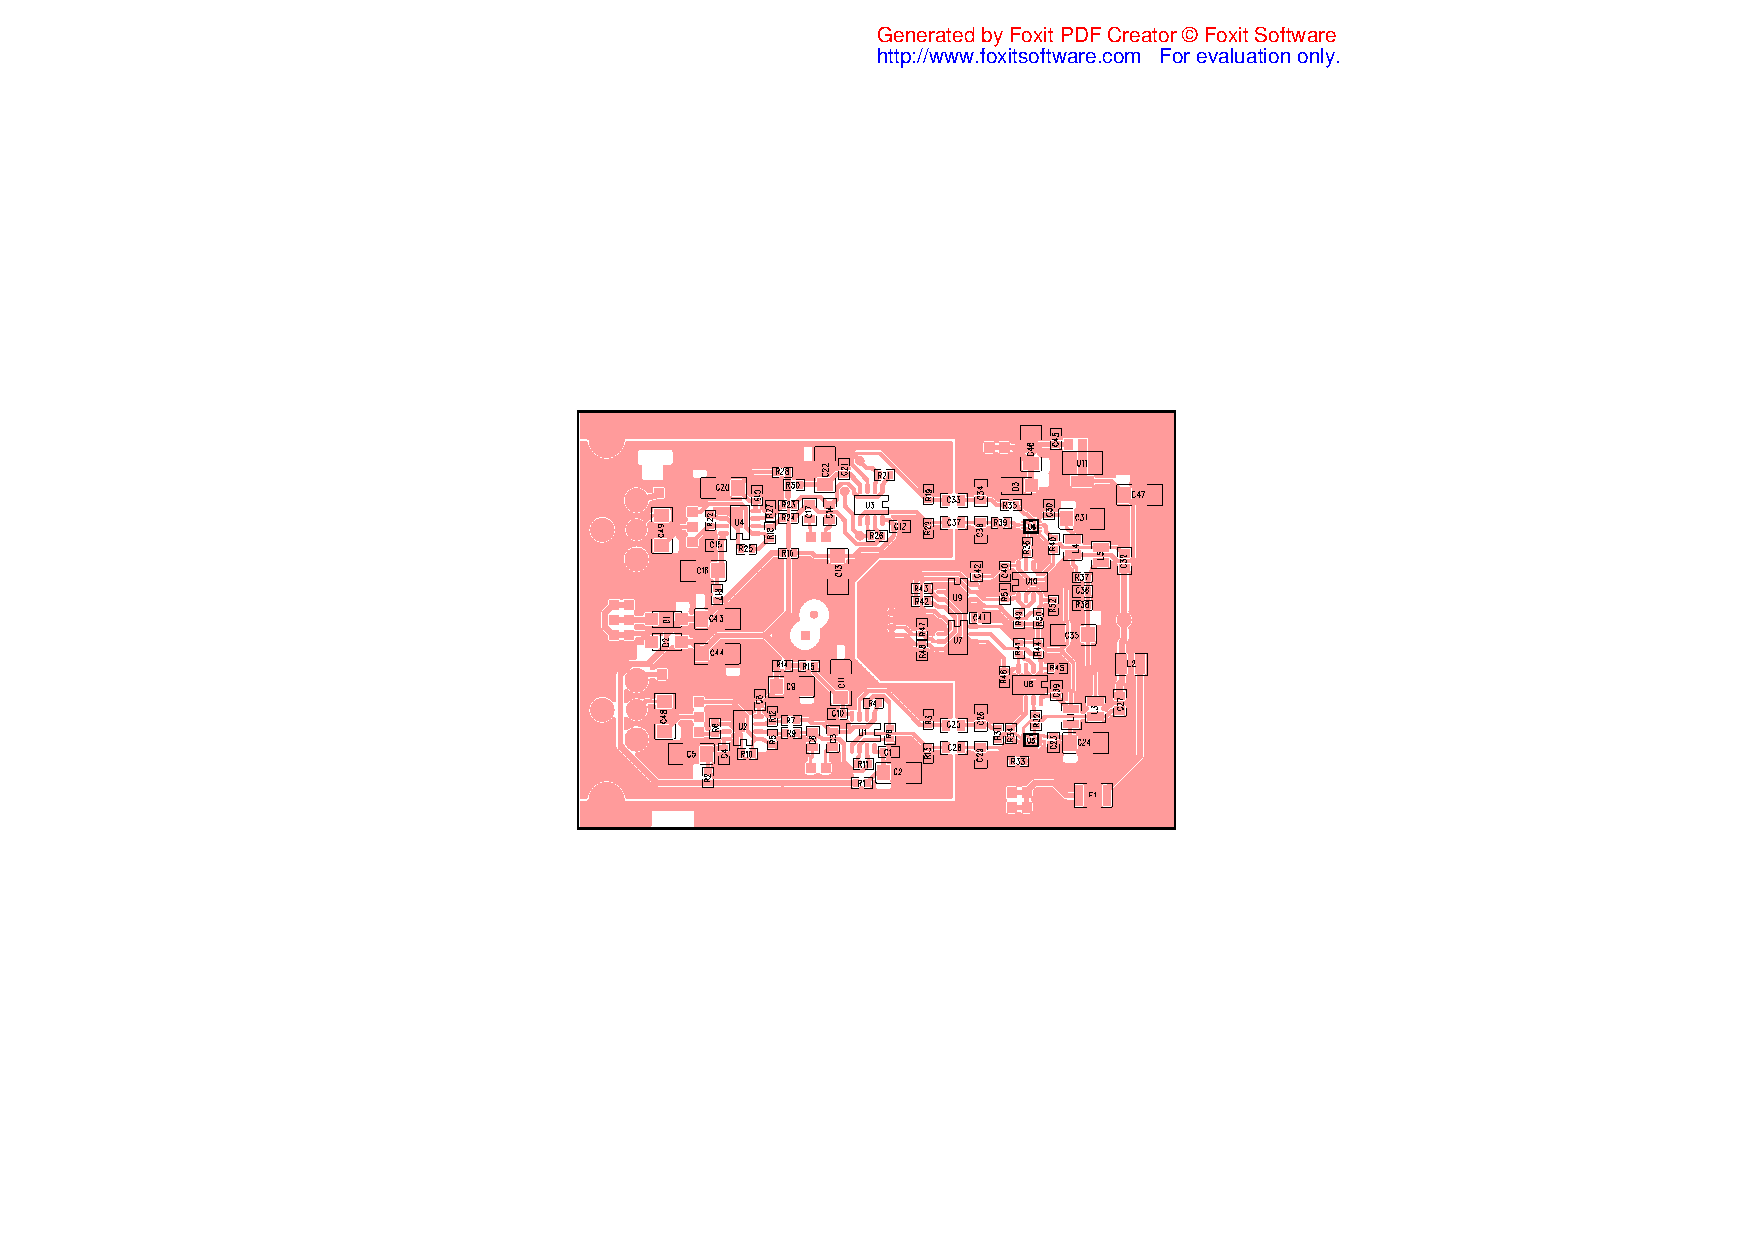
\includepdf[pages={1},landscape=true]{../../CAM_DOC/O2.pdf}

\subsection{EMI suppression}
For proper function of receiver is necessary to use proper low noise symmetric power supply (classical PC power supply is unacceptable). There is need for proper routing of grounding wires, which must be routed in star topology. In addition there is few jumpers on the board of receiver to allow proper selection of ground connection.

\subsection{Mechanical construction}

The mechanical construction of the receiver resulted (For better EMI suppression is suggested use of metal MLAB base such as ALBASE). Two layer PCB is chosen mainly because of better shielding by top cooper layer and even because better grounding. In case where long term stability is required receiver must be inserted to thermostatic box together with LO. 

\subsubsection{Setting}
There is one easy step for proper setting of the receiver. The trimmer P1 must be tunned to value where the strength of mirror frequencies is minimized or zero. This can be achieved by tunning the receiver to some strength AM transmitter and slowly turning by P1 until the mirror of signal in frequency spectrum is minimized. 

\section{Software tools}

The basic software tools for this receiver are all programs designed to work with sound card as I/Q input. Such as Winrad, WinradHD or Spectrum Lab. There is usually request to add a LO library for tunning Si570, but tunning the LO by separate software is acceptable too.

\begin{thebibliography}{99}
\bibitem{DR2G}{The original construction of DR2G} 
\href{http://yu1lm.qrpradio.com/SMT SDR RX DR2G-YU1LM.pdf}{http://yu1lm.qrpradio.com/SMT SDR RX DR2G-YU1LM.pdf}

\end{thebibliography}
\end{document}